\chapter{Addestramento e confronto dei modelli}
\label{ch:training-and-comparison}

Il \Cref{ch:forecasting-models} ha definito la GCN e le baseline con cui confrontarne le prestazioni da un punto di vista prettamente teorico, senza stabilire come ogni modello venga addestrato o come le sue previsioni siano giudicate. Questo capitolo sviluppa il protocollo \emph{walk-forward} di addestramento e validazione e i test di significatività statistica sui confronti tra modelli.

\section{Insidie della validazione}
\label{sec:tc-pitfalls}

La pipeline del caso di studio seleziona la procedura di \emph{training} evitando errori metodologici che falserebbero le prestazioni della stima. L'errore misurato sul blocco di test è una stima di quello che il modello commetterebbe in un impiego reale, distorta verso l'ottimismo ogni volta che il protocollo concede al modello informazioni che in quell'impiego non avrebbe. Sui rendimenti finanziari, dove il rapporto segnale-rumore è basso, questa distorsione può superare in ampiezza il segnale stesso. Si distinguono le seguenti insidie ricorrenti.

\subsection{Look-ahead bias}

Consiste nell'usare informazione non ancora disponibile alla chiusura del giorno $t$ per prevedere $r_{t+1}$. Si verifica anche in operazioni come la standardizzazione delle feature: calcolare media e deviazione standard sull'intero campione, addestramento e test insieme, inietta nel modello informazioni sulla distribuzione futura dei dati. La pipeline non fallisce, ma i risultati migliorano in modo silenzioso.

\subsection{Data snooping}

Si realizza quando gli stessi dati sono usati sia per scegliere che per valutare un modello. È probabile che, tra molte configurazioni prive di capacità predittiva provate sullo stesso blocco di test, almeno una batta il riferimento per puro caso: il suo vantaggio è un effetto della selezione e cresce con il numero di configurazioni provate. Il \enquote{Reality Check} di \textcite{white2000reality} ne tiene conto confrontando il modello migliore non con il riferimento, ma con il miglior risultato che l'insieme dei modelli provati otterrebbe per caso. La pipeline di progetto impedisce il \emph{data snooping} fissando in anticipo la griglia della GCN (\cref{sec:tc-gcn-training}) e correggendo i test multipli del confronto finale con il metodo di Holm (\cref{sec:tc-significance}).

\subsection{Validazione incrociata su serie temporali}

La $k$-fold \emph{cross-validation} suddivide i dati in $k$ blocchi, addestrando il modello $k$ volte, ciascuna su $k-1$ blocchi, e valutandolo su quello escluso. Su una serie temporale, il modello viene addestrato anche su osservazioni successive a quelle su cui è valutato, violando l'ordine temporale che incontrerebbe in un impiego reale.

\section{Il protocollo walk-forward}
\label{sec:tc-walkforward}

La validazione walk-forward ovvia al problema della $k$-fold rispettando l'ordine temporale dei dati. Il modello viene addestrato su una finestra di osservazioni e valutato sul periodo immediatamente successivo. La finestra avanza rispetto all'inizio della precedente, ripetendo poi la procedura. Ogni valutazione avviene quindi su dati posteriori a quelli di training. Nello studio, il modello si colloca alla chiusura del giorno $t$ e prevede $r_{t+1}$ utilizzando le sole osservazioni fino a $t$ compreso.

\subsection{La finestra causale}

Per evitare che, all'origine $t$, il modello includa anche la riga $t+1$, il rendimento da prevedere, ogni input dei modelli è estratto da \texttt{causal\_windows}. Questa funzione si occupa di aggiungere, in testa al pannello, $\texttt{window}-1$ righe di \texttt{NaN} e di ricavare, con \texttt{sliding\_window\_view}, tutte le finestre consecutive. A partire da un pannello $(T, N)$, come quello dei rendimenti $r\in\mathbb{R}^{2006\times 15}$ ricavato alla \cref{sec:returns-stationarity}, si ottiene un tensore $(T, \texttt{window}, N)$.

\begin{listing}[H]
\begin{minted}{python}
def causal_windows(values: np.ndarray, window: int) -> np.ndarray:
    if values.ndim != 2:
        raise ValueError(f"Expected a (T, N) panel, got {values.ndim} dimensions")
    if window < 1:
        raise ValueError(f"Window must be at least 1, got {window}")
    if window > len(values):
        raise ValueError(f"Window of {window} exceeds the {len(values)} rows available")

    pad = np.full((window - 1, values.shape[1]), np.nan)
    padded = np.vstack([pad, values])
    return sliding_window_view(padded, window, axis=0).transpose(0, 2, 1)
\end{minted}
\caption{\texttt{causal\_windows}}
\label{lst:causal-windows}
\end{listing}

Per ogni riga $t$ il risultato contiene le \texttt{window} righe che terminano in $t$, in ordine cronologico: \texttt{result[t, -1]} è la riga $t$ stessa e \texttt{result[t, -1 - k]} la riga $t-k$. Le prime righe del risultato, prive di una storia completa, contengono \texttt{NaN}.

\subsection{Le feature dei nodi}
\label{sec:tc-node-features}

Le finestre causali trovano il loro primo utilizzo nel calcolo delle $F=8$ feature, dette anche canali, che la GCN riceve in ingresso per ciascun nodo e ciascuna origine $t$. Sono ricavate dai pannelli dei rendimenti e dei volumi (\cref{sec:returns-stationarity}) e descrivono tre aspetti diversi del comportamento recente di un asset: il suo andamento, il suo rischio e l'attività di scambio. Fissata l'origine, esse formano la matrice $H^{(0)}\in\mathbb{R}^{N\times F}$ \eqref{eq:gcn}, con una riga per ciascuno dei $15$ asset e una colonna per canale.

I primi cinque canali sono i rendimenti ritardati $r_t, r_{t-1}, \dots, r_{t-4}$. Rappresentano la dinamica di breve periodo del prezzo. Il rendimento $r_t$ è incluso perché noto alla chiusura del giorno in cui si prevede. Il sesto e il settimo canale sono la volatilità realizzata su $5$ e $20$ giorni, cioè l'ampiezza tipica dei rendimenti recenti. Rappresentano il livello di rischio corrente dell'asset e riflettono il volatility clustering (\cref{sec:stylized-facts}). L'ottavo canale confronta il logaritmo del volume scambiato nel giorno $t$ con la sua media sugli ultimi $20$ giorni, $t$ compreso, espresso in deviazioni standard. Un volume insolitamente alto segnala in genere l'arrivo di nuova informazione o un cambiamento nell'interesse degli operatori, e accompagna spesso i movimenti di prezzo più ampi. Prima di essere usate nella GCN, le feature sono standardizzate separatamente in ciascun fold (\cref{sec:tc-single-training}).

\subsection{La geometria dei fold}

Lo studio usa uno schema walk-forward di tipo \emph{rolling} con $24$ fold. I fold vengono ricavati direttamente dal pannello dei rendimenti $r$ (\cref{sec:returns-stationarity}): ognuno di essi è costituito da un training set di $365$ \emph{entry}, un validation set di $63$ entry ed un test set di $63$ entry. Il fold successivo ha inizio $63$ righe dopo l'inizio del precedente: l'addestramento mantiene in questo modo una lunghezza fissa e i blocchi di test di fold consecutivi si affiancano senza sovrapporsi.

Il primo fold parte dalla posizione $T_w-1=59$, perché prima della sessantesima osservazione non esiste alcun grafo di correlazione (\cref{sec:correlation-matrix-to-graph}). I fold vengono aggiunti fino a quando il successivo non supera l'ultima riga utilizzabile per prevedere $r_{t+1}$, ovvero la penultima riga del pannello. Il periodo di test va dal 05/05/2022 al 24/06/2026, per $1512$ giorni e $22\,680$ previsioni per modello sui $15$ asset.

Ogni fold, al momento della sua costruzione, verifica che i tre insiemi siano non vuoti, formati da righe consecutive del pannello e disposti nell'ordine training, validation, test; in caso contrario l'esecuzione si interrompe con un errore.

\begin{figure}[H]
\centering
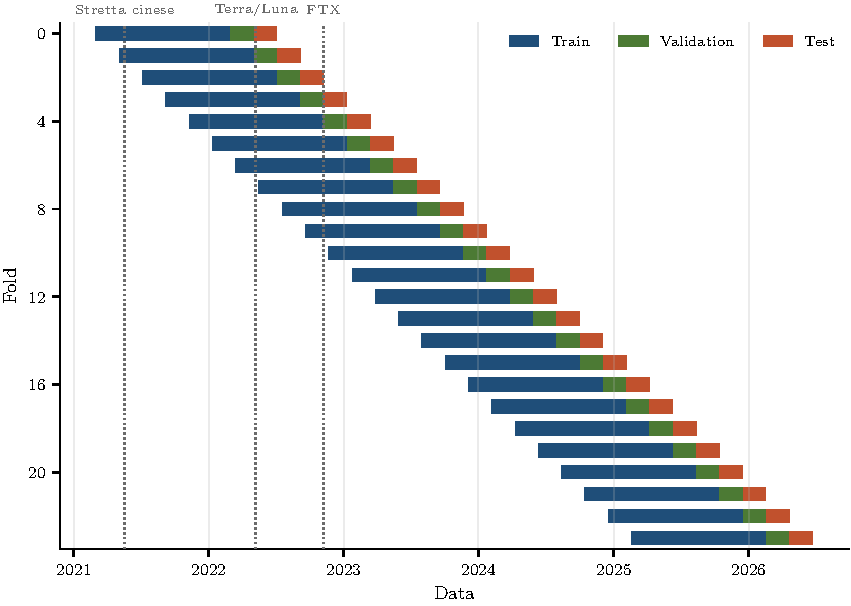
\includegraphics[width=\textwidth]{figures/fig_walkforward_scheme.pdf}
\caption[Schema del protocollo walk-forward]{I $24$ fold del protocollo walk-forward, con addestramento, validazione e test e le date dei tre eventi di crisi. La stretta cinese del 19/05/2021 precede il periodo previsto e compare solo nell'analisi topologica della \cref{sec:topo-event-study}; Terra/Luna e FTX cadono dentro un blocco di test e sono valutate fuori campione.}
\label{fig:tc-walkforward-scheme}
\end{figure}

\subsection{Target del test set}

I modelli utilizzati nello studio (\cref{ch:forecasting-models}) ricevono, per ciascun fold, tre oggetti \texttt{Segment}, uno per blocco (train, validation, test), con le sole righe del blocco corrispondente. La riga $i$ di un segmento contiene rendimenti, feature e adiacenza $\hat A$ all'origine $t_i$, il target $y_i=r_{t_i+1}$ e i ritardi più recenti fino a $t_i$ compreso, ricavati da \texttt{causal\_windows}. I ritardi sono distinti dalle feature: sono i rendimenti nelle loro unità originali, senza standardizzazione, e costituiscono l'ingresso delle baseline autoregressive, che stimano i propri coefficienti direttamente su questi ultimi. Nel blocco di test il target non deve essere accessibile al modello: il metodo \texttt{without\_target} è utilizzato a tal proposito.

\begin{listing}[H]
\begin{minted}{python}
def without_target(self) -> Segment:
    return replace(self, y=np.full_like(self.y, np.nan))
\end{minted}
\caption{\texttt{without\_target}}
\label{lst:without-target}
\end{listing}

Esso restituisce una copia del segmento in cui \texttt{y} è sostituito da \texttt{NaN}. Si impedisce quindi il \emph{data leakage}.

\subsection{Il ciclo di valutazione}

Ogni modello del progetto implementa \texttt{fit(train, val)} e \texttt{predict(segment)}. I modelli che non utilizzano la validazione ricevono comunque \texttt{val} e lo ignorano. Questa firma unica permette a \texttt{run\_walkforward} (\cref{lst:run-walkforward}) di trattare tutti i modelli con lo stesso codice.

Per ciascun fold, \texttt{run\_walkforward} costruisce i tre oggetti \texttt{Segment} e interrompe l'esecuzione se uno di essi contiene feature o adiacenze non finite, segno di un fold che risale a posizioni prive di grafo. Crea poi un modello nuovo tramite \texttt{factory} per ogni fold, affinché i parametri stimati per quello precedente non vengano riutilizzati nel successivo. Il modello viene addestrato su \texttt{train\_segment} e \texttt{val\_segment}, e prevede su \texttt{test\_segment.without\_target()}.

La funzione restituisce un oggetto \texttt{WalkforwardResult}, composto da due tabelle. La prima, \texttt{predictions}, raccoglie le previsioni del solo blocco di test in formato lungo: una riga per fold, data, asset e modello, con il rendimento realizzato \texttt{y\_true} e quello previsto \texttt{y\_pred}. La seconda, \texttt{diagnostics}, contiene una riga per fold con le dimensioni dei tre blocchi e il tempo di addestramento.

\begin{longlisting}{\texttt{run\_walkforward}}{lst:run-walkforward}
\begin{minted}{python}
def run_walkforward(factory: Callable[[], Forecaster], data: WalkforwardData, folds: list[Fold], name: str | None = None, verbose: bool = True) -> WalkforwardResult:

    predictions: list[pd.DataFrame] = []
    diagnostics: list[dict[str, object]] = []
    n_assets = data.n_assets
    assets = np.asarray(data.assets)

    for fold in folds:
        _validate_fold(data, fold)
        train_segment = data.segment(fold.train)
        val_segment = data.segment(fold.val)
        test_segment = data.segment(fold.test)
        for segment, split in ((train_segment, "train"), (val_segment, "val"), (test_segment, "test")):
            _check_finite(segment, fold, split)

        model = factory()
        model_name = name if name is not None else getattr(model, "name", type(model).__name__)

        started = time.perf_counter()
        model.fit(train_segment, val_segment)
        fit_seconds = time.perf_counter() - started

        predicted = np.asarray(model.predict(test_segment.without_target()), dtype=float)
        if predicted.shape != (len(test_segment), n_assets):
            raise ValueError(
                f"Fold {fold.index}: {model_name} predicted {predicted.shape}, "
                f"expected {(len(test_segment), n_assets)}"
            )
        if not np.isfinite(predicted).all():
            raise ValueError(f"Fold {fold.index}: {model_name} produced non-finite predictions")

        predictions.append(
            pd.DataFrame(
                {
                    "fold": fold.index,
                    "date": test_segment.target_dates.repeat(n_assets),
                    "asset": np.tile(assets, len(test_segment)),
                    "y_true": test_segment.y.ravel(),
                    "y_pred": predicted.ravel(),
                    "model": model_name,
                }
            )
        )

        n_train, n_val, n_test = fold.sizes
        row: dict[str, object] = {
            "fold": fold.index,
            "model": model_name,
            "n_train": n_train,
            "n_val": n_val,
            "n_test": n_test,
            "fit_seconds": fit_seconds,
        }
        if isinstance(model, SupportsDiagnostics):
            row.update(model.diagnostics())
        diagnostics.append(row)

        if verbose:
            # Print the fold's block sizes, test dates and fit time.
            ...

    return WalkforwardResult(
        predictions=pd.concat(predictions, ignore_index=True),
        diagnostics=pd.DataFrame(diagnostics),
    )
\end{minted}
\end{longlisting}

Le previsioni delle baseline sono salvate su disco prima dell'addestramento della GCN e successivamente rilette senza essere ricalcolate. Il termine di confronto è in questo modo fissato prima che sia noto il risultato del modello da valutare.

L'assenza di look-ahead (\cref{sec:tc-pitfalls}) è verificata da test dedicati. Si controllano, in particolare, l'ordine dei blocchi di ciascun fold, l'allineamento del grafo, verificando che quello usato per prevedere $r_{t+1}$ sia costruito sui soli rendimenti in $[t-59,t]$, la standardizzazione delle feature (\cref{sec:tc-single-training}) e l'assenza di $r_{t+1}$ in ciascuna di esse. Sui grafi, infatti, la verifica è immediata, poiché è sufficiente dimostrare che $\hat A$ non contenga il rendimento del giorno successivo.

\section{Addestramento della GCN}
\label{sec:tc-gcn-training}

La GCN, a differenza delle baseline del \Cref{ch:forecasting-models}, stimate in forma chiusa o con un criterio di selezione, deve essere addestrata per discesa del gradiente (\cref{sec:from-perceptron-to-graph-layer}): i pesi $W^{(l)}$ e i bias $b^{(l)}$ dell'equazione~\eqref{eq:gcn} sono spostati ripetutamente nella direzione da esso indicata. L'addestramento della rete introduce quindi quattro scelte che le baseline non richiedono: in che forma i dati raggiungono la rete, con quale regola i pesi vengono aggiornati, per quanto a lungo e con quali valori degli iperparametri che il gradiente non tocca. La configurazione è fissata a priori.

\subsection{Gli ingressi della rete}
\label{sec:tc-single-training}

La GCN è l'unico modello dello studio che legge entrambi i tensori dell'oggetto \texttt{Segment}: le feature dei nodi (\cref{sec:tc-node-features}) e le adiacenze $\hat A$ (\cref{sec:correlation-matrix-to-graph}).

Le feature sono standardizzate prima di raggiungere la rete. Media e deviazione standard sono stimate per asset e per canale sul solo blocco di addestramento, e applicate invariate a validazione e test. Stimarle sul solo training evita il look-ahead della \cref{sec:tc-pitfalls}. Stimarle per asset risponde invece alla condivisione dei pesi della \cref{sec:gcn-kipf-welling}: la matrice $W^{(l)}$ è la stessa per tutti i nodi e gli asset differiscono in volatilità fino a un ordine di grandezza.

Il target è invece diviso per un unico scalare $s$, la deviazione standard dei rendimenti di addestramento. I pesi iniziali sono estratti da un intervallo calibrato perché la varianza del segnale si conservi da uno strato al successivo: poiché le feature hanno ormai varianza unitaria, una rete non addestrata restituisce valori di ordine uno, contro rendimenti dell'ordine di $0{,}04$. Senza la divisione, le prime epoche servirebbero solo a ridurre la scala dell'uscita. Lo scalare è unico per l'intero pannello: dividere per una costante moltiplica il costo per $1/s^2$ senza spostarne il minimo. Previsioni ed errori tornano poi in unità di rendimento.

Le adiacenze sono infine allineate al pannello da \texttt{align\_graph}. Il grafo esiste solo dalla sessantesima osservazione (\cref{sec:correlation-matrix-to-graph}), quindi il tensore è più corto di $T_w-1$ righe. Ogni matrice è collocata sulla riga della data in cui la sua finestra si chiude, garantendo che l'adiacenza in posizione $t$ sia costruita sui soli rendimenti fino a $t$. Le righe prive di grafo sono riempite di \texttt{NaN}, non di zeri: un'adiacenza nulla addestrerebbe il modello su un mercato senza relazioni, mentre il \texttt{NaN} si propaga e viene intercettato da \texttt{run\_walkforward} (\cref{sec:tc-walkforward}).

\begin{listing}[H]
\begin{minted}{python}
def align_graph(a_hat: np.ndarray, corr_index: pd.DatetimeIndex, dates: pd.DatetimeIndex) -> np.ndarray:
    # Check the graph tensor and the correlation index have the same length.
    ...
    panel = pd.DatetimeIndex(dates)
    graph_dates = pd.DatetimeIndex(corr_index)
    # Reconcile the timezone of the two indices.
    ...

    positions = panel.get_indexer(graph_dates)
    if (positions < 0).any():
        missing = graph_dates[positions < 0]
        raise ValueError(f"{len(missing)} correlation dates absent from the return panel, first {missing[0]}")

    aligned = np.full((len(dates), *a_hat.shape[1:]), np.nan, dtype=float)
    aligned[positions] = a_hat
    return aligned
\end{minted}
\caption{\texttt{align\_graph}}
\label{lst:align-graph}
\end{listing}

Il tensore restituito ha tante matrici quante sono le righe del pannello, e ciascuna occupa la posizione della propria data di chiusura. Le date del grafo assenti dal pannello ricevono da \texttt{get\_indexer} la posizione $-1$ e interrompono l'esecuzione: le due sorgenti devono descrivere lo stesso periodo perché una posizione $t$ abbia un unico significato.

\subsection{Adam e la regolarizzazione}

Il criterio di aggiornamento dei pesi che la pipeline utilizza è Adam~\cite{kingmaba2015adam}, applicato all'errore quadratico medio (MSE): ogni parametro riceve un passo di dimensione propria, ricavato dalla storia dei suoi gradienti.

Per ciascun parametro $w$ l'ottimizzatore conserva due medie mobili esponenziali, aggiornate a ogni passo $k$ a partire dal gradiente $g_k$ del costo rispetto a $w$
\begin{equation}
\label{eq:adam-moments}
m_k = \beta_1 m_{k-1} + (1-\beta_1)\,g_k, \qquad v_k = \beta_2 v_{k-1} + (1-\beta_2)\,g_k^2.
\end{equation}
La prima memoria, $m_k$, è la media dei gradienti recenti e ne rappresenta la direzione prevalente: se i gradienti di passi successivi concordano, i loro contributi si sommano e il passo accelera; se si alternano di segno, si elidono a vicenda e il passo si accorcia. La seconda, $v_k$, è la media dei loro quadrati e misura l'ampiezza tipica del gradiente di quel parametro, indipendentemente dal segno. I coefficienti $\beta_1$ e $\beta_2$ fissano la lunghezza delle due memorie, ovvero la rapidità con cui il passato viene dimenticato.

Il passo effettivo del parametro si ricava dalle due memorie
\begin{equation}
\label{eq:adam-update}
w_k = w_{k-1} - \eta\,\frac{\hat m_k}{\sqrt{\hat v_k}+\varepsilon}, \qquad \hat m_k = \frac{m_k}{1-\beta_1^k}, \qquad \hat v_k = \frac{v_k}{1-\beta_2^k}.
\end{equation}
Le versioni $\hat m_k$ e $\hat v_k$ correggono le due memorie dalla distorsione dovuta all'inizializzazione a zero, che altrimenti le sottostimerebbe nei primi passi. Dividendo la prima per la radice della seconda si ottiene un passo che non dipende più dalla scala del gradiente, ma soltanto dalla sua costanza; $\varepsilon$ impedisce la divisione per zero; $\eta$ è il passo base, unico per tutti i parametri.

Il vantaggio rispetto alla discesa del gradiente a passo fisso (\cref{sec:from-perceptron-to-graph-layer}) emerge quando una direzione è molto più ripida dell'altra (\cref{fig:tc-adam-vs-gd}). A passo fisso, l'unico $\eta$ disponibile deve essere sufficientemente piccolo da non far divergere la direzione ripida. La traiettoria oscilla allora tra i due versanti della valle, avanzando lentamente lungo il suo fondo. Con Adam, invece, la discesa segue esattamente il fondo della valle.

\begin{figure}[H]
\centering
\begin{subfigure}{\textwidth}
\centering
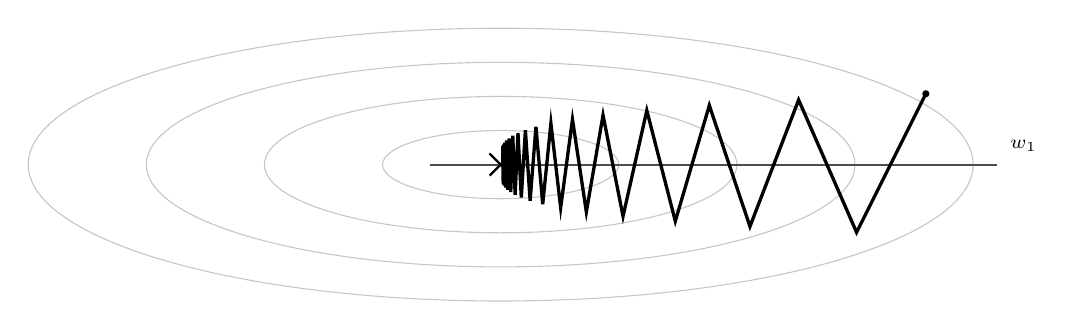
\begin{tikzpicture}[x=2.0cm, y=2.0cm, every node/.style={font=\small}]
    \foreach \r in {0.75, 1.5, 2.25, 3.0} {
        \draw[gray!45] (0,0) ellipse ({\r} and {\r/3.464});
    }
    \draw[black!70, thick] (-0.45,0) -- (3.15,0);
    \node[font=\scriptsize] at (3.32,0.12) {$w_1$};
    \draw[very thick]
        (2.700,0.450) -- (2.260,-0.430) -- (1.892,0.411) -- (1.583,-0.393) -- (1.325,0.376) --
        (1.109,-0.359) -- (0.928,0.344) -- (0.777,-0.328) -- (0.650,0.314) -- (0.544,-0.300) --
        (0.456,0.287) -- (0.381,-0.274) -- (0.319,0.262) -- (0.267,-0.251) -- (0.224,0.240) --
        (0.187,-0.229) -- (0.157,0.219) -- (0.131,-0.209) -- (0.110,0.200) -- (0.092,-0.191) --
        (0.077,0.183) -- (0.064,-0.175) -- (0.054,0.167) -- (0.045,-0.160) -- (0.038,0.153) --
        (0.032,-0.146) -- (0.026,0.140) -- (0.022,-0.134) -- (0.019,0.128) -- (0.016,-0.122) --
        (0.013,0.117);
    \fill (2.700,0.450) circle (1.3pt);
    \draw[thick] (-0.07,-0.07) -- (0.07,0.07) (-0.07,0.07) -- (0.07,-0.07);
\end{tikzpicture}
\caption{Discesa del gradiente a passo fisso}
\label{fig:tc-adam-vs-gd-a}
\end{subfigure}

\vspace{12pt}

\begin{subfigure}{\textwidth}
\centering
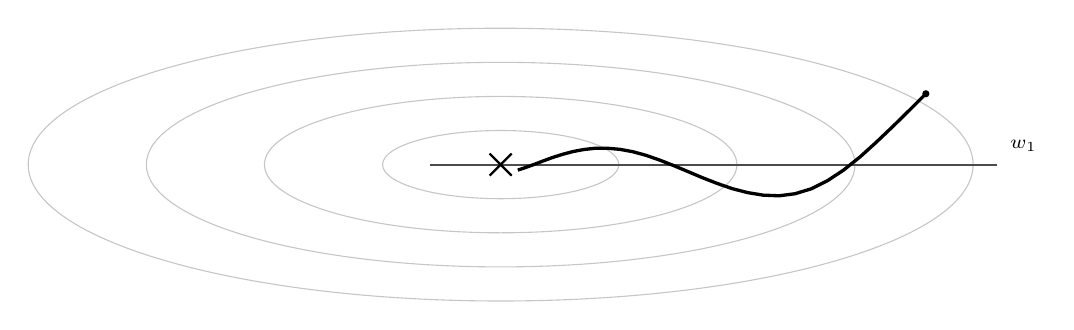
\begin{tikzpicture}[x=2.0cm, y=2.0cm, every node/.style={font=\small}]
    \foreach \r in {0.75, 1.5, 2.25, 3.0} {
        \draw[gray!45] (0,0) ellipse ({\r} and {\r/3.464});
    }
    \draw[black!70, thick] (-0.45,0) -- (3.15,0);
    \node[font=\scriptsize] at (3.32,0.12) {$w_1$};
    \draw[very thick]
        (2.700,0.450) -- (2.595,0.345) -- (2.490,0.242) -- (2.385,0.142) -- (2.281,0.048) --
        (2.177,-0.035) -- (2.074,-0.103) -- (1.971,-0.154) -- (1.869,-0.185) -- (1.768,-0.198) --
        (1.668,-0.194) -- (1.569,-0.178) -- (1.472,-0.153) -- (1.376,-0.120) -- (1.281,-0.083) --
        (1.189,-0.044) -- (1.098,-0.006) -- (1.009,0.029) -- (0.923,0.059) -- (0.839,0.082) --
        (0.757,0.097) -- (0.678,0.104) -- (0.602,0.104) -- (0.529,0.096) -- (0.459,0.083) --
        (0.392,0.065) -- (0.329,0.045) -- (0.269,0.023) -- (0.212,0.001) -- (0.159,-0.018) --
        (0.109,-0.035);
    \fill (2.700,0.450) circle (1.3pt);
    \draw[thick] (-0.07,-0.07) -- (0.07,0.07) (-0.07,0.07) -- (0.07,-0.07);
\end{tikzpicture}
\caption{Adam}
\label{fig:tc-adam-vs-gd-b}
\end{subfigure}
\caption[Discesa del gradiente e Adam a confronto]{Trenta passi dei due metodi sulla stessa funzione di costo quadratica $C(w_1,w_2)=\tfrac12\left(w_1^2+12\,w_2^2\right)$, a partire dallo stesso punto. Le ellissi sono le curve di livello di $C$, la croce il suo minimo e il punto la posizione iniziale. La direzione $w_2$ è dodici volte più ripida di $w_1$.}
\label{fig:tc-adam-vs-gd}
\end{figure}

Si applicano due meccanismi per limitare l'adattamento al rumore del blocco di addestramento. Il primo è il \emph{weight decay}, fissato a $0{,}0005$, che ad ogni passo riduce leggermente la norma dei pesi, penalizzando le soluzioni di ampiezza elevata. Il secondo è il \emph{dropout}~\cite{srivastava2014dropout}: durante l'addestramento ciascuna componente del tensore in ingresso ad uno strato è azzerata con probabilità $p$, indipendentemente dalle altre, riscalando le componenti superstiti affinché la somma resti della stessa ampiezza. Nell'architettura a due strati della \cref{sec:known-limitations-gnn}, il dropout è applicato prima di ciascuno dei due ed è attivo soltanto in fase di training: in valutazione, la rete è deterministica e usa tutte le componenti. L'addestramento è \emph{full-batch}. Ogni epoca corrisponde quindi ad un solo passo di Adam, calcolato su tutte le origini del blocco.

\subsection{Epoche ed early stopping}

Il numero di epoche dipende dal singolo fold. Il ciclo di \texttt{fit} ne esegue al più $300$ e affida al blocco di validazione la decisione di fermarsi prima.

\begin{listing}[H]
\begin{minted}{python}
for epoch in range(1, self.epochs + 1):
    model.train()
    optimizer.zero_grad()
    criterion(model(train_a, train_x), train_y).backward()
    optimizer.step()
    in_returns = self.target_scale_**2
    model.eval()
    with torch.no_grad():
        val_mse = float(criterion(model(val_a, val_x), val_y)) * in_returns
    if val_mse < best_val:
        best_val, best_epoch = val_mse, epoch
        best_state = copy.deepcopy(model.state_dict())
        waited = 0
    else:
        waited += 1
        if waited >= self.patience:
            break
model.load_state_dict(best_state)
\end{minted}
\caption{\texttt{fit}}
\label{lst:gcn-fit}
\end{listing}

Dopo ogni passo di ottimizzazione l'errore è ricalcolato in modalità \texttt{eval}, cioè senza dropout, perché la quantità su cui si decide deve essere quella della rete che verrà poi usata per prevedere. Se l'MSE di validazione migliora, i pesi correnti sono copiati e il contatore di attesa azzerato; se non migliora per $30$ epoche consecutive l'addestramento si arresta. Questa procedura prende il nome di \emph{early stopping}.

Senza il ripristino di \texttt{best\_state} il modello conservato sarebbe quello di $30$ epoche successive al minimo, strettamente peggiore del migliore osservato e da esso indistinguibile in qualunque log. I semi casuali, infine, sono fissati all'inizio di \texttt{fit} e non nel costruttore, così che rieseguire un singolo fold riproduca esattamente il risultato che quel fold ha prodotto nell'esecuzione completa.

\subsection{La griglia e la selezione}

Gli iperparametri che intervengono nell'addestramento della GCN e che il gradiente non tocca sono due, e costituiscono una griglia fissata prima di osservare qualunque risultato. Le \emph{hidden units} valgono $16$ o $32$: è la dimensione interna delle due matrici dell'equazione~\eqref{eq:gcn}, cioè la larghezza della rappresentazione $H^{(1)}$, e quindi la capacità del modello. Il dropout vale invece $0{,}2$ o $0{,}5$. La profondità resta fissa a due strati. Fissare la griglia risponde al data snooping della \cref{sec:tc-pitfalls}: il numero di configurazioni provate è dichiarato in anticipo e non cresce dopo aver visto il blocco di test.

Si ottengono quindi quattro configurazioni, ciascuna delle quali è addestrata, per ogni fold, con $5$ semi diversi per la generazione casuale dei pesi iniziali. I semi non aggiungono un terzo asse, perché non si sceglie tra loro: le $5$ reti di una stessa configurazione sono mediate e la previsione della configurazione è la media delle loro previsioni. Il criterio di selezione che ne segue è l'MSE di validazione della media delle $5$ previsioni e non la media dei $5$ MSE. La quantità su cui si sceglie coincide così con quella che il blocco di test misurerà, e la previsione finale del fold è quella della sola configurazione selezionata. Anche le previsioni di validazione, infine, sono richieste su un segmento privato del target, alle stesse condizioni del test. Sui $24$ fold e sui due bracci della \cref{sec:tc-ablation} lo studio addestra quindi $960$ reti.

\begin{table}[H]
\centering
\caption[MSE di validazione sulla griglia GCN]{MSE di validazione medio sui $24$ fold per ciascuna cella della griglia fissata, per i due bracci dell'ablation.}
\label{tab:tc-gcn-grid}
\small
\begin{tabular*}{\textwidth}{@{\extracolsep{\fill}}rrrr@{}}
\toprule
\textbf{Hidden units} & \textbf{Dropout} & \textbf{GCN} & \textbf{GCN senza grafo} \\
\midrule
$16$ & $0{,}2$ & $0{,}001726$ & $0{,}001745$ \\
$16$ & $0{,}5$ & $0{,}001725$ & $0{,}001736$ \\
$32$ & $0{,}2$ & $0{,}001725$ & $0{,}001738$ \\
$32$ & $0{,}5$ & $0{,}001725$ & $0{,}001733$ \\
\bottomrule
\end{tabular*}
\end{table}

\begin{table}[H]
\centering
\caption[Esito della selezione sulla griglia GCN]{Configurazione più spesso selezionata sui $24$ fold, con il suo MSE di validazione, le epoche medie di addestramento e la quota di addestramenti interrotti dall'early stopping.}
\label{tab:tc-gcn-selection}
\small
\begin{tabular*}{\textwidth}{@{\extracolsep{\fill}}lcrrr@{}}
\toprule
\textbf{Braccio} & \textbf{Configurazione} & \textbf{MSE val.} & \textbf{Epoche} & \textbf{Early stop} \\
\midrule
GCN & $h{=}16,\,p{=}0{,}5$ ($9/24$) & $0{,}001706$ & $66{,}7$ & $100{,}0\%$ \\
GCN senza grafo & $h{=}32,\,p{=}0{,}2$ ($9/24$) & $0{,}001720$ & $91{,}8$ & $98{,}3\%$ \\
\bottomrule
\end{tabular*}
\end{table}

Nella \cref{tab:tc-gcn-grid} le quattro celle della GCN coincidono fino alla quinta cifra decimale, e il vantaggio del braccio con grafo su quello senza, pur presente in ogni cella, non supera la dispersione interna alla griglia del braccio senza grafo. La selezione non distingue meglio: i due bracci non convergono sulla stessa configurazione più frequente e ciascuna delle due si aggiudica appena $9$ fold su $24$ (\cref{tab:tc-gcn-selection}), con un MSE che, essendo un minimo scelto fold per fold, non è confrontabile con le medie della tabella precedente. Una griglia così piatta è coerente con l'assenza di un segnale predittivo più che con un'esplorazione insufficiente.

\section{Lo studio di ablation}
\label{sec:tc-ablation}

Confrontare la GCN con le baseline di riferimento non è sufficiente per isolare il contributo del grafo. La rete neurale, infatti, differisce dai modelli autoregressivi anche per le feature di ingresso, per la non linearità e per la procedura di addestramento. Un eventuale vantaggio potrebbe dipendere da uno di questi fattori. Uno studio di ablation rimuove una sola componente del modello, lasciando invariato tutto il resto. Nel progetto, la componente rimossa è l'adiacenza $\hat A$, sostituita con la matrice identità $I$ prima di applicare i due layer.

Con $\hat A=I$ l'equazione~\eqref{eq:gcn} si riduce a $H^{(l+1)}=\sigma\bigl(H^{(l)}W^{(l)}+b^{(l)}\bigr)$, un percettrone applicato a ciascun nodo separatamente con gli stessi pesi. L'unica differenza tra i due bracci riguarda la considerazione delle informazioni dei vicini. I due bracci sono costruiti da \texttt{gcn\_factories}.

\begin{listing}[H]
\begin{minted}{python}
def gcn_factories(config: Config) -> dict[str, Callable[[], GCNGridForecaster]]:
    return {
        name: lambda use_graph=use_graph: GCNGridForecaster(config, use_graph=use_graph)
        for name, use_graph in (("gcn", True), ("gcn-nograph", False))
    }
\end{minted}
\caption{\texttt{gcn\_factories}}
\label{lst:gcn-factories}
\end{listing}

I due bracci sono poi eseguiti, come le baseline, attraverso \texttt{run\_walkforward}. Il confronto tra \texttt{gcn} e \texttt{gcn-nograph} è la forma più diretta della prima questione di ricerca posta nell'Introduzione. Il suo esito è riportato nella \cref{sec:tc-results}.

\section{Lo skill score}
\label{sec:tc-skill-score}

La \cref{sec:baselines} ha osservato che la previsione nulla $\hat r_{t+1,a}=0$ si colloca, sui rendimenti giornalieri, vicino all'errore quadratico medio minimo raggiungibile. L'errore di un modello, preso singolarmente, non fornisce sufficiente informazione. Sul periodo di test dello studio, la previsione nulla ha un RMSE di $0{,}04145$. Si giudicano gli altri modelli rispetto a questo valore. Lo skill score rende esplicito il confronto
\begin{equation}
\label{eq:skill-score}
\mathrm{skill} = 1-\frac{\mathrm{MSE}_{\text{modello}}}{\mathrm{MSE}_{\text{zero}}},
\end{equation}
e rappresenta la frazione dell'errore quadratico della previsione nulla che il modello riesce a muovere. Lo skill score vale $0$ per un modello equivalente alla previsione nulla; è positivo quando il modello la batte e negativo in caso contrario, senza alcun limite inferiore. Il valore massimo $1$ corrisponde ad una previsione perfetta del modello confrontato.

\begin{listing}[H]
\begin{minted}{python}
def skill_score(y: np.ndarray, pred: np.ndarray, baseline_pred: np.ndarray) -> float:
    baseline_mse = float(np.mean((np.asarray(y) - np.asarray(baseline_pred)) ** 2))
    if baseline_mse <= 0:
        raise ValueError("Baseline MSE is zero: the skill score is undefined against a perfect reference")
    return 1.0 - float(np.mean((np.asarray(y) - np.asarray(pred)) ** 2)) / baseline_mse
\end{minted}
\caption{\texttt{skill\_score}}
\label{lst:skill-score}
\end{listing}

Accanto allo skill score il progetto riporta, per ogni modello, RMSE, MAE e accuratezza direzionale, intesa come la frazione di previsioni con segno corretto. Quest'ultima esclude le coppie in cui il rendimento o la previsione valgono esattamente zero: una previsione esattamente nulla non esprime alcuna direzione e contarla come errata attribuirebbe alla baseline \texttt{ZeroForecaster} un'accuratezza pari a zero. Insieme all'accuratezza si restituisce la copertura, ovvero la quota di coppie su cui l'accuratezza è stata calcolata.

\begin{listing}[H]
\begin{minted}{python}
def directional_accuracy(y: np.ndarray, pred: np.ndarray) -> tuple[float, float]:
    y = np.asarray(y)
    pred = np.asarray(pred)
    taken = (y != 0) & (pred != 0)
    coverage = float(taken.mean()) if taken.size else 0.0

    if not taken.any():
        return float("nan"), coverage
    return float((np.sign(y[taken]) == np.sign(pred[taken])).mean()), coverage
\end{minted}
\caption{\texttt{directional\_accuracy}}
\label{lst:directional-accuracy}
\end{listing}

\section{Significatività del confronto}
\label{sec:tc-significance}

La differenza di skill score tra due modelli è una stima calcolata su un campione finito: sugli stessi $1512$ giorni di test può riflettere un vantaggio reale, oppure il rumore del particolare periodo osservato. Nei dati dello studio, sei dei sette modelli si collocano entro l'$1{,}6\%$ di MSE dalla previsione nulla, il che rende necessario un test che stabilisca se una differenza sia distinguibile o meno dalla fluttuazione campionaria.

\subsection{Il test di Diebold-Mariano}

Il test di \textcite{dieboldmariano1995comparing} confronta l'accuratezza di due previsioni $a$ e $b$ tramite il differenziale di perdita $d_t=e_{a,t}^2-e_{b,t}^2$. Sotto l'ipotesi nulla di pari accuratezza, il suo valore atteso è nullo. La statistica è la media campionaria di $d_t$, divisa per il suo errore standard. Per previsioni ad un passo, come quelle dello studio, si scrive
\begin{equation}
\label{eq:diebold-mariano}
\mathrm{DM}=\sqrt{\frac{n-1}{n}}\;\frac{\bar d}{\sqrt{\hat\sigma_d^2/n}},\qquad \bar d=\frac1n\sum_{t=1}^n d_t,
\end{equation}
dove $\hat\sigma_d^2$ è la varianza campionaria di $d_t$. Per un orizzonte $h=1$ il differenziale di una previsione ottima non è autocorrelato e la varianza campionaria è sufficiente. Il fattore $\sqrt{\frac{n-1}{n}}$ è la correzione per campioni finiti di \textcite{harvey1997testing}. La statistica corretta si confronta con una $t$ di Student a $n-1$ gradi di libertà. Per costruzione $\mathrm{DM}$ è negativa quando il modello $a$ è il più accurato dei due.

\begin{longlisting}{\texttt{\_newey\_west\_variance} e \texttt{diebold\_mariano}}{lst:diebold-mariano}
\begin{minted}{python}
def _newey_west_variance(d: np.ndarray, lags: int) -> float:
    centered = d - d.mean()
    n = len(d)
    variance = float(np.dot(centered, centered) / n)
    for lag in range(1, lags + 1):
        covariance = float(np.dot(centered[lag:], centered[:-lag]) / n)
        variance += 2.0 * (1.0 - lag / (lags + 1.0)) * covariance
    return variance


def diebold_mariano(errors_a: np.ndarray, errors_b: np.ndarray, h: int = 1) -> DieboldMariano:
    # Check the shape of the two error series and the horizon.
    ...
    d = errors_a**2 - errors_b**2
    n = len(d)
    if n <= h:
        raise ValueError(f"Need more than h = {h} observations to test, got {n}")
    variance = _newey_west_variance(d, lags=h - 1)
    if variance <= 0:
        raise ValueError(
            "Non-positive long-run variance of the loss differential: the two models "
            "most likely produced identical errors, in which case there is nothing to test"
        )

    statistic = d.mean() / np.sqrt(variance / n)
    correction = np.sqrt((n + 1 - 2 * h + h * (h - 1) / n) / n)
    statistic *= correction

    return DieboldMariano(
        statistic=float(statistic),
        p_value=float(2.0 * stats.t.sf(abs(statistic), df=n - 1)),
        df=n - 1,
        mean_loss_differential=float(d.mean()),
    )
\end{minted}
\end{longlisting}

La funzione implementa la forma generale della correzione,
$$\sqrt{\frac{n+1-2h+\frac{h(h-1)}{n}}{n}},$$
che per $h=1$ si riduce al fattore dell'equazione~\eqref{eq:diebold-mariano}. Per $h>1$ il differenziale è autocorrelato e la varianza campionaria va sostituita da una stima di Newey-West con $h-1$ ritardi. Con $h=1$ il ciclo di \texttt{\_newey\_west\_variance} non viene eseguito. Il $p$-value è bilaterale.

\subsection{Il differenziale sul pannello}

Resta da stabilire su quali errori calcolare $d_t$. Ogni modello produce $22\,680$ previsioni, ma i rendimenti delle criptovalute si muovono insieme e con essi gli errori di qualunque modello che li segua. L'errore standard dell'equazione~\eqref{eq:diebold-mariano} presuppone osservazioni distinte, mentre i $15$ asset di una stessa giornata portano in buona parte la stessa informazione: contarli separatamente lo sottostimerebbe. Il progetto calcola quindi, per ciascuna data, l'errore quadratico medio sui $15$ asset e applica il test alla serie giornaliera di $1512$ osservazioni.

\begin{listing}[H]
\begin{minted}{python}
def panel_loss_differential(predictions: pd.DataFrame, model_a: str, model_b: str) -> tuple[np.ndarray, np.ndarray]:
    frame = predictions[predictions["model"].isin([model_a, model_b])].copy()
    frame["squared_error"] = (frame["y_true"] - frame["y_pred"]) ** 2
    daily = frame.groupby(["model", "date"])["squared_error"].mean().unstack("model")
    for model in (model_a, model_b):
        if model not in daily.columns:
            raise ValueError(f"No predictions for model {model!r}")
    aligned = daily[[model_a, model_b]].dropna()
    return np.sqrt(aligned[model_a].to_numpy()), np.sqrt(aligned[model_b].to_numpy())
\end{minted}
\caption{\texttt{panel\_loss\_differential}}
\label{lst:panel-loss-differential}
\end{listing}

La media è calcolata sugli errori al quadrato e non sugli errori: errori di segno opposto su due asset si compenserebbero altrimenti in una giornata apparentemente perfetta. La funzione restituisce la radice dell'errore quadratico medio giornaliero, che \texttt{diebold\_mariano} eleva di nuovo al quadrato.

\subsection{La correzione di Holm}

Il confronto a coppie di sette modelli comporta $\binom72=21$ test. Se ciascuno di essi è condotto al livello del $5\%$, anche in assenza di qualunque differenza reale ci si attende in media un rifiuto per effetto del solo numero di test, conseguenza diretta del data snooping (\cref{sec:tc-pitfalls}). La procedura di \textcite{holm1979simple} controlla il FWER, ovvero la probabilità di commettere almeno un falso rifiuto nell'intera famiglia di test. Ordinati gli $m$ $p$-value in modo crescente, $p_{(1)}\leq\dots\leq p_{(m)}$, il $p$-value corretto del $k$-esimo è
\begin{equation}
\label{eq:holm}
\tilde p_{(k)}=\min\Bigl(1,\ \max_{j\leq k}\,(m-j+1)\,p_{(j)}\Bigr).
\end{equation}
Confrontare $\tilde p_{(k)}$ con il livello $\alpha$ equivale alla procedura sequenziale originale.

\begin{listing}[H]
\begin{minted}{python}
def holm_adjusted(p_values: np.ndarray) -> np.ndarray:
    # Check the array is one-dimensional and not empty.
    ...
    order = np.argsort(p_values)
    ranked = p_values[order] * (len(p_values) - np.arange(len(p_values)))
    adjusted = np.empty_like(ranked)
    adjusted[order] = np.minimum(np.maximum.accumulate(ranked), 1.0)
    return adjusted
\end{minted}
\caption{\texttt{holm\_adjusted}}
\label{lst:holm-adjusted}
\end{listing}

La correzione è necessaria perché lo studio non esegue un test soltanto. Il $p$-value di un singolo confronto misura quanto sarebbe improbabile la differenza osservata se i due modelli fossero equivalenti; ripetuto sulle $21$ coppie distinte al livello del $5\%$, quel margine di errore si accumula e almeno un confronto supera la soglia per il solo effetto del rumore. Senza correzione, la tabella dei risultati offrirebbe ventuno occasioni di dichiarare un modello migliore, senza alcun modo di distinguere un vantaggio reale da uno prodotto dal rumore. La correzione è applicata sulle $21$ coppie non ordinate e non sulle $42$ righe della matrice di Diebold-Mariano, che contengono ciascun test due volte e ne raddoppierebbero il conteggio; viene poi riportata su entrambe le direzioni di ogni coppia. La famiglia comprende tutte le coppie e non i soli confronti con la previsione nulla.

\section{Risultati}
\label{sec:tc-results}

L'accuratezza dei sette modelli è riportata in tre scomposizioni, complessiva, per asset e per fold, tutte prodotte dalla stessa funzione \texttt{summarize\_predictions}: il calcolo è quindi identico nelle tre viste e per tutti i modelli, e le differenze che emergono sono attribuibili ai dati e non alla procedura che li riassume.

\begin{listing}[H]
\begin{minted}{python}
def summarize_predictions(predictions: pd.DataFrame, baseline: str = "zero", by: str | Sequence[str] | None = None) -> pd.DataFrame:
    # Check the baseline is present and the grouping keys exist.
    ...
    keys = [by] if isinstance(by, str) else list(by or [])
    reference = predictions[predictions["model"] == baseline].set_index(["date", "asset"])["y_pred"]

    rows = []
    for values, group in predictions.groupby(["model", *keys], sort=False):
        labels = dict(zip(["model", *keys], values if isinstance(values, tuple) else (values,), strict=True))
        indexed = group.set_index(["date", "asset"])
        baseline_pred = reference.reindex(indexed.index)
        if baseline_pred.isna().any():
            raise ValueError(f"Model {labels['model']!r} covers dates or assets the baseline {baseline!r} does not")

        rows.append(labels | _accuracy_row(indexed, baseline_pred))

    return pd.DataFrame(rows).sort_values([*keys, "rmse"], ignore_index=True)
\end{minted}
\caption{\texttt{summarize\_predictions}}
\label{lst:summarize-predictions}
\end{listing}

Nelle scomposizioni lo skill score~\eqref{eq:skill-score} è calcolato all'interno di ciascun gruppo contro le previsioni nulle dello stesso. Lo skill di un modello su BTC misura quindi il miglioramento rispetto a prevedere zero su BTC, non rispetto all'intero pannello. Le due quantità differiscono ogni volta che la volatilità varia tra i gruppi, come accade su questi dati.

\subsection{Accuratezza complessiva}

La scomposizione complessiva riunisce in un'unica tabella le misure di accuratezza della \cref{sec:tc-skill-score} e il test della \cref{sec:tc-significance}. RMSE e MAE misurano l'ampiezza dell'errore, l'accuratezza direzionale il solo segno e lo skill score la posizione del modello rispetto alla previsione nulla; la statistica DM e il suo $p$ corretto stabiliscono se quella posizione sia distinguibile dalla fluttuazione campionaria.

\begin{table}[H]
\centering
\caption[Confronto predittivo tra i modelli]{Accuratezza fuori campione sui $22\,680$ valori previsti del periodo di test, ordinata per RMSE crescente. La statistica DM confronta ciascun modello con la previsione nulla ed è negativa quando il modello è il più accurato dei due. Il $p$ è corretto secondo Holm sull'insieme dei $21$ confronti a coppie. L'accuratezza direzionale della previsione nulla non è definita.}
\label{tab:tc-results-main}
\small
\begin{tabular}{@{}lrrrrrr@{}}
\toprule
\textbf{Modello} & \textbf{RMSE} & \textbf{MAE} & \textbf{Acc. dir.} & \textbf{Skill} & \textbf{DM} & \textbf{$p$ (Holm)} \\
\midrule
Zero & $0{,}04145$ & $0{,}02764$ & -- & $0{,}0000$ & -- & -- \\
Media storica & $0{,}04156$ & $0{,}02773$ & $50{,}0\%$ & $-0{,}0052$ & $2{,}78$ & $0{,}077$ \\
VAR (BIC) & $0{,}04156$ & $0{,}02773$ & $50{,}0\%$ & $-0{,}0052$ & $2{,}78$ & $0{,}077$ \\
GCN senza grafo & $0{,}04162$ & $0{,}02776$ & $51{,}2\%$ & $-0{,}0080$ & $1{,}59$ & $1{,}000$ \\
AR & $0{,}04162$ & $0{,}02774$ & $50{,}4\%$ & $-0{,}0082$ & $3{,}36$ & $0{,}012$ \\
GCN & $0{,}04177$ & $0{,}02801$ & $50{,}9\%$ & $-0{,}0156$ & $1{,}82$ & $0{,}683$ \\
VAR ($p=5$) & $0{,}04978$ & $0{,}03471$ & $50{,}1\%$ & $-0{,}4423$ & $11{,}00$ & $<0{,}001$ \\
\bottomrule
\end{tabular}
\end{table}

La \Cref{tab:tc-results-main} ordina i sette modelli per RMSE crescente. Nessun modello batte la previsione nulla. Lo skill score è negativo per tutti gli altri modelli, da $-0{,}0052$ della media storica a $-0{,}4423$ del VAR con ordine fissato. Tutte le statistiche DM sono positive. Dopo la correzione di Holm solo due modelli risultano significativamente \emph{peggiori} della previsione nulla, l'AR ($p_{\mathrm{Holm}}=0{,}012$) e il VAR con $p=5$ ($p_{\mathrm{Holm}}<0{,}001$). La media storica e il VAR selezionato per BIC, numericamente identici, restano al limite ($p_{\mathrm{Holm}}=0{,}077$). La GCN e la sua ablation non si distinguono dalla previsione nulla ($p_{\mathrm{Holm}}=0{,}683$ e $1{,}000$).

Il VAR con ordine fissato rende concreto il problema di sovraparametrizzazione della \cref{sec:var-baseline}. Con $4{,}8$ osservazioni per parametro il modello si adatta al rumore del blocco di addestramento. Fuori campione il suo RMSE sale da $0{,}04145$ a $0{,}04978$. L'accuratezza direzionale resta tra il $50{,}0\%$ e il $51{,}2\%$ per tutti i modelli. Anche sul segno nessun modello si discosta in modo apprezzabile da una scelta casuale.

\subsection{L'esito dell'ablation}

Il confronto che risponde più direttamente alla prima questione di ricerca è quello tra i due bracci dell'ablation. Il test di Diebold-Mariano tra \texttt{gcn} e \texttt{gcn-nograph} restituisce $\mathrm{DM}=1{,}338$, con $p=0{,}181$ e $p_{\mathrm{Holm}}=1{,}000$. Il segno positivo indica che la GCN con il grafo è la meno accurata delle due, con un differenziale medio di perdita pari a $1{,}296\cdot10^{-5}$. Il $p$-value indica che la differenza non è distinguibile dal rumore, tanto meno dopo la correzione. Il grafo non peggiora in modo dimostrabile la previsione, ma non vi è alcuna evidenza che la migliori.

\subsection{Eterogeneità tra asset}

La media sul pannello nasconde le differenze tra i quindici asset, che si distinguono in volatilità fino a un ordine di grandezza.

\begin{table}[H]
\centering
\caption[Skill score per asset]{Skill score contro la previsione nulla dello stesso asset, per i due bracci della GCN.}
\label{tab:tc-skill-by-asset}
\small
\begin{tabular}{@{}lrr@{}}
\toprule
\textbf{Asset} & \textbf{GCN} & \textbf{GCN senza grafo} \\
\midrule
ADA & $-0{,}0134$ & $-0{,}0057$ \\
AVAX & $-0{,}0109$ & $-0{,}0072$ \\
BCH & $-0{,}0209$ & $-0{,}0055$ \\
BNB & $-0{,}0347$ & $-0{,}0084$ \\
BTC & $-0{,}0557$ & $-0{,}0329$ \\
DOGE & $-0{,}0038$ & $0{,}0053$ \\
DOT & $-0{,}0087$ & $-0{,}0069$ \\
ETC & $-0{,}0138$ & $-0{,}0057$ \\
ETH & $-0{,}0307$ & $-0{,}0177$ \\
LINK & $-0{,}0089$ & $-0{,}0112$ \\
LTC & $-0{,}0202$ & $-0{,}0183$ \\
SOL & $-0{,}0051$ & $-0{,}0070$ \\
TRX & $-0{,}0468$ & $-0{,}0150$ \\
XLM & $-0{,}0099$ & $-0{,}0069$ \\
XRP & $-0{,}0148$ & $-0{,}0043$ \\
\bottomrule
\end{tabular}
\end{table}

La \Cref{tab:tc-skill-by-asset} scompone per asset lo skill score dei due bracci. Su $30$ celle, $15$ asset per $2$ bracci, una sola è positiva, quella della variante senza grafo su DOGE ($+0{,}0053$). Entrambi i bracci ottengono lo skill peggiore su BTC, con $-0{,}0557$ e $-0{,}0329$. La GCN è meno accurata della propria ablation su $13$ asset su $15$, con le sole eccezioni di LINK e SOL.

\subsection{Eterogeneità tra fold}

La media sull'intero periodo nasconde una forte variabilità. La \Cref{fig:tc-results-by-fold} scompone lo skill score fold per fold. La GCN ottiene uno skill positivo in $9$ fold su $24$, più di ogni altro modello. Seguono la variante senza grafo con $7$ fold, la media storica e il VAR selezionato per BIC con $6$, l'AR con $2$ e il VAR con ordine fissato con $0$. Tra i due bracci la GCN ha tuttavia lo skill complessivo peggiore. Le due osservazioni non sono in contraddizione: lo skill complessivo è calcolato sugli errori quadratici dell'intero periodo e non sul numero di fold favorevoli, e la penalità quadratica amplifica i pochi fold in cui la GCN sbaglia di più, fino a compensare i margini contenuti dei fold in cui prevale.

\begin{figure}[H]
\centering
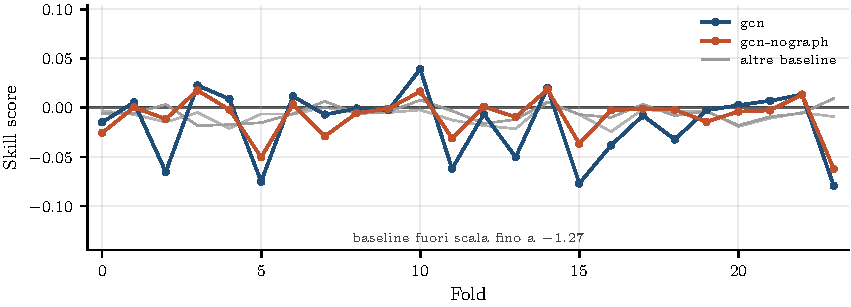
\includegraphics[width=\textwidth]{figures/fig_results_by_fold.pdf}
\caption[Skill score per fold]{Skill score contro la previsione nulla, fold per fold, per i due bracci della GCN e le baseline. La scala verticale è calibrata sui due bracci evidenziati. Le baseline che escono dall'intervallo sono annotate con il loro valore peggiore.}
\label{fig:tc-results-by-fold}
\end{figure}

\subsection{Densità del grafo e skill score}

La \Cref{sec:known-limitations-gnn} ha osservato che su un grafo denso l'over-smoothing si manifesta a profondità minore. Il \Cref{ch:topological-evolution} ha mostrato che il grafo dello studio è quasi completo e che si compatta attorno alle crisi. Si verifica quindi un'ipotesi che incrocia le due questioni di ricerca, ovvero se nei fold in cui il grafo è più denso la GCN preveda peggio.

Questa associazione è misurata dalla correlazione di rango di Spearman. La scelta del coefficiente è motivata da due ragioni fondamentali: l'ipotesi afferma una monotonicità e non una forma funzionale, che è esattamente ciò che una correlazione di rango quantifica; e alla soglia calibrata $8$ fold su $24$ hanno densità media esattamente pari a $1$, un blocco di pari merito a cui i ranghi assegnano il rango medio, con una spaziatura unitaria che limita l'influenza dei fold più distanti.

La retta mostrata nella \cref{fig:tc-density-vs-error} è la stima di Theil-Sen, cioè la mediana delle pendenze tra coppie di punti. Il risultato è $\rho=-0{,}100$ ($p=0{,}643$) alla soglia calibrata e $\rho=0{,}005$ ($p=0{,}981$) alla soglia $\tau_{\mathrm{FWER}}$, dove nessun fold satura. Nessuna delle due associazioni è distinguibile da zero, esito interpretabile come un test a bassa potenza e non come una confutazione. Alla soglia calibrata, inoltre, la densità media per fold varia solo tra $0{,}887$ e $1{,}000$, comprimendo proprio la variazione di cui il test avrebbe bisogno.

\begin{figure}[H]
\centering
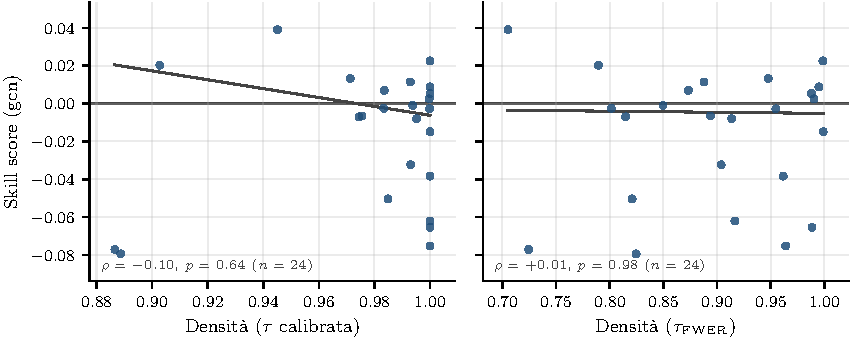
\includegraphics[width=\textwidth]{figures/fig_density_vs_error.pdf}
\caption[Densità del grafo e skill score della GCN]{Skill score della GCN contro la densità media del grafo nel blocco di test, per fold, alle soglie $\tau$ e $\tau_{\mathrm{FWER}}$. La retta è la stima di Theil-Sen.}
\label{fig:tc-density-vs-error}
\end{figure}

Il protocollo walk-forward, la griglia fissata a priori e la correzione per confronti multipli lasciano poco margine per orientare il confronto verso un esito favorevole. L'esito è negativo: nessuno dei sei modelli batte la baseline \texttt{ZeroForecaster} sui rendimenti giornalieri, e la GCN non si distingue in modo statisticamente significativo né da essa né dalla propria ablation senza grafo.
